\chapter{Exploratory Analysis of Foursquare Dataset}

\section{Task 1-3}

\begin{enumerate}
    \item Use \verb|SparkContext.textFile| to read in checkins and countries to RDDs.
    \item Use the \verb|map| functions in \verb|task1/mappers.py| to manipulate each row of the data input. Remove first row, split on tab and convert to object (\verb|record_to_object|), calculate local time (\verb|calculate_local_time|), assign a city the naive way (\verb|find_nearest_city_and_country|, iterating through the entire list of countries for each checkin).
    \item Persist the result for further usage. 
    
\end{enumerate}

\section{Task 4}
\begin{enumerate}
    \item \verb|map| the wanted key (\verb|user_id|, \verb|checkin_id|, etc.)
    \item Use \verb|distinct| to remove all duplicates.
    \item Use \verb|count| to get the length of the RDD. 
\end{enumerate}

This gave the following results:
\begin{description}
    \item[(a) How many unique users are represented in the dataset?] \hfill \\
        Number of distinct user IDs : 256307
    \item[(b) How many times did they check-in in total?] \hfill  \\
        Number of total checkins: 19265256
    \item[(c) How many check-in sessions are there in the dataset?] \hfill  \\
        Number of distinct session IDs : 6338302
    \item[(d) How many countries are represented in the dataset?]\hfill  \\
        Number of distinct country : 77
    \item[(e) How many cities are represented in the dataset?]\hfill  \\
        Number of distinct cities : 413
\end{description}



\section{Task 5}


\begin{enumerate}
    \item \verb|map| \verb|session_id| as key, and 1 as value.
    \item Use \verb|reduceByKey(lambda a, b: a + b)| to accumulate the number of checkins per session.
    \item \verb|map| the session lengths as key, and 1 as value.
    \item Use \verb|reduceByKey| again to find lengths of sessions as number of checkins.
    \item \verb|saveAsTextFile| to write the result to disk. 
\end{enumerate}
    
We used Google Spreadsheets to produce a histogram with occurrences of session lengths as seen in figure \ref{fig:histogram}.
\begin{figure}
\centering
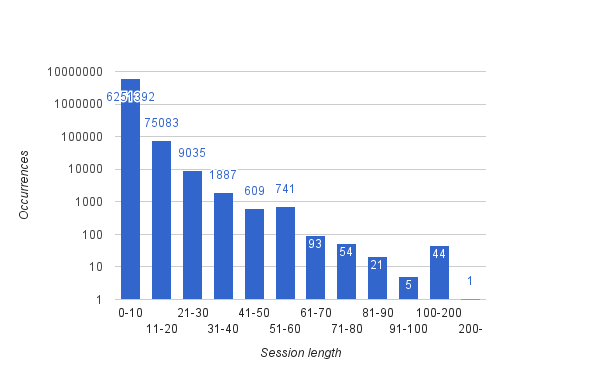
\includegraphics[height=10cm]{figs/image.png}
\caption{Histogram showing the number of occurrences of grouped session lengths. Logarithmic scale.}
\label{fig:histogram}
\end{figure}



\section{Task 6-7}

A screenshot from CartoDB can be seen in figure \ref{fig:cartodb}. The map can be further explored \href{https://esso.cartodb.com/viz/dbcd3dce-063e-11e6-b0d7-0e8c56e2ffdb/public_map}{here}.
\begin{figure}
\centering
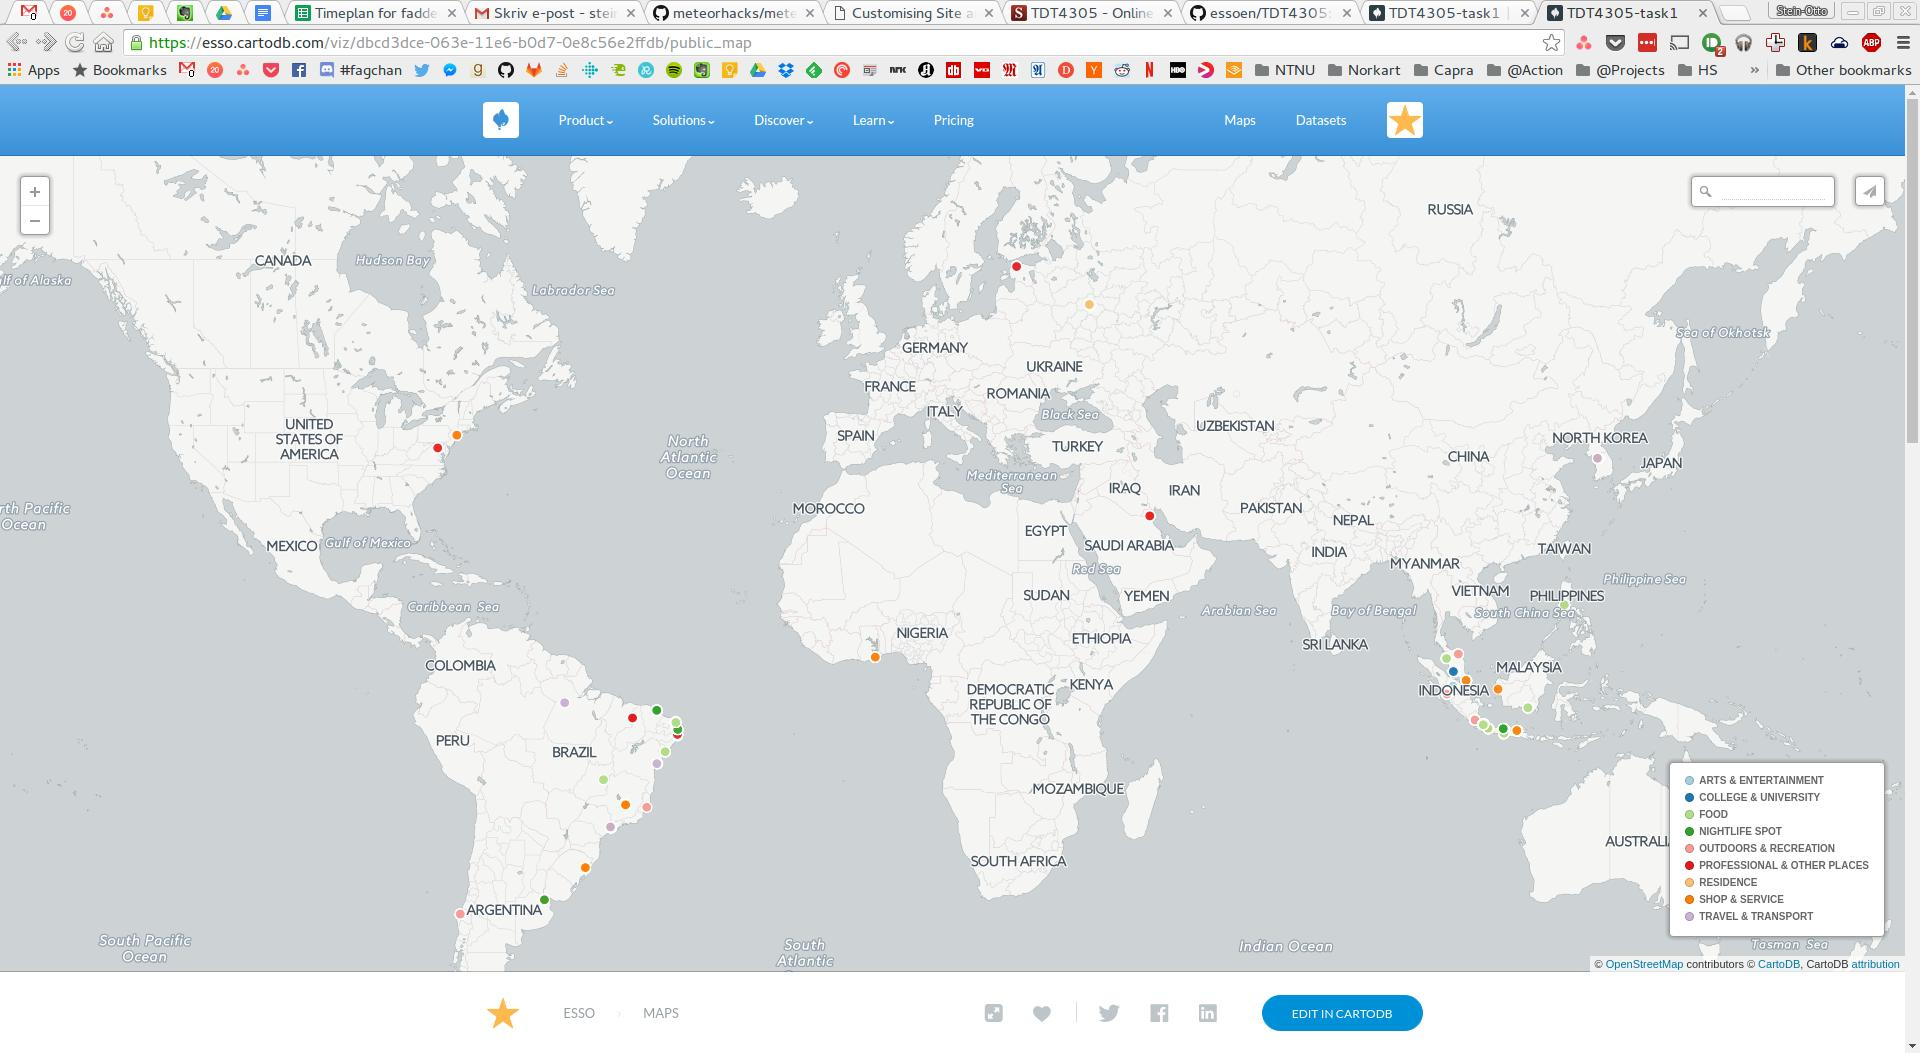
\includegraphics[height=10cm]{figs/cartodb.jpg}
\caption{Screenshot of the map produced with CartoDB.}
\label{fig:cartodb}
\end{figure}

\begin{enumerate}
    \item \verb|map| \verb|session_id| as key, and the rest as value.
    \item \verb|groupByKey| to get an iterator per \verb|session_id|.
    \item \verb|mapValues(lambda o: list(o)| to get a list per \verb|session_id|.
    \item \verb|filter| out every list with length less than 4. 
    \item \verb|map| in the session distance (\verb|calculate_session_distance|) as a third tuple element.
    \item \verb|filter| out sessions with distance smaller than 50.
    \item Use \verb|takeOrdered(100, key=lambda o: -len(o[1])| to return a list with the 100 longest sessions.
    \item Open a result file, and write tab separated values to disk again. 
\end{enumerate}


